% This file was created by tikzplotlib vunknown.
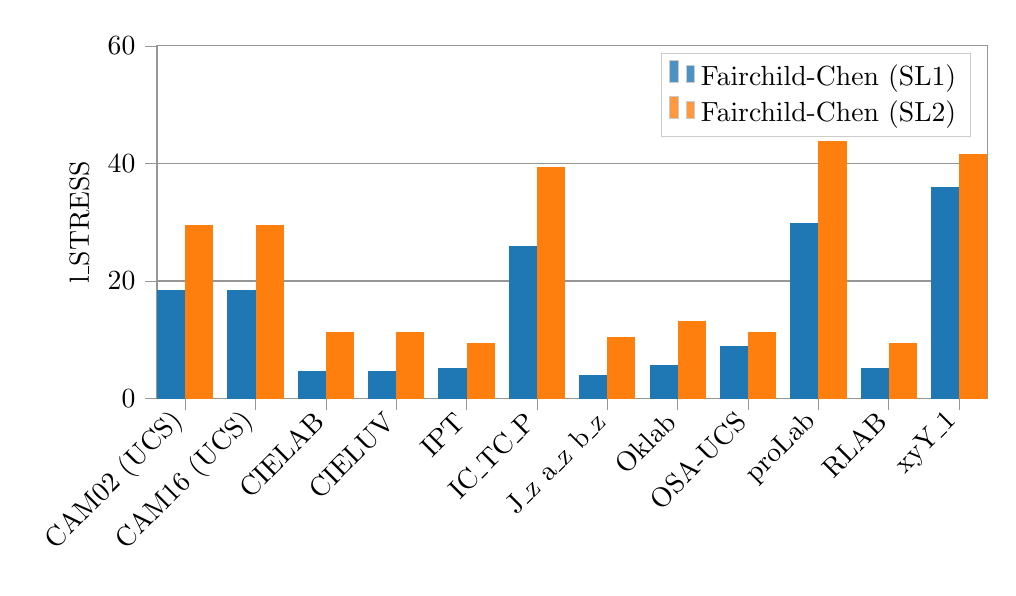
\begin{tikzpicture}

\definecolor{color0}{rgb}{0.12156862745098,0.466666666666667,0.705882352941177}
\definecolor{color1}{rgb}{1,0.498039215686275,0.0549019607843137}

\begin{axis}[
axis line style={white!58.8235294117647!black},
height=0.5\textwidth,
legend cell align={left},
legend style={fill opacity=0.8, draw opacity=1, text opacity=1, draw=white!80!black},
tick align=outside,
tick pos=left,
width=\textwidth,
x grid style={white!58.8235294117647!black},
xmin=-0.4, xmax=11.4,
xtick style={color=white!58.8235294117647!black},
xtick={0,1,2,3,4,5,6,7,8,9,10,11},
xticklabel style={rotate=45.0,anchor=east},
xticklabels={CAM02 (UCS),CAM16 (UCS),CIELAB,CIELUV,IPT,IC\_TC\_P,J\_z a\_z b\_z,Oklab,OSA-UCS,proLab,RLAB,xyY\_1},
y grid style={white!58.8235294117647!black},
ylabel={l\_STRESS},
ymajorgrids,
ymin=0, ymax=60,
ytick style={color=white!58.8235294117647!black}
]
\draw[draw=none,fill=color0] (axis cs:-0.4,0) rectangle (axis cs:0,18.4645911268359);
\addlegendimage{ybar,ybar legend,draw=none,fill=color0};
\addlegendentry{Fairchild-Chen (SL1)}

\draw[draw=none,fill=color0] (axis cs:0.6,0) rectangle (axis cs:1,18.462147583011);
\draw[draw=none,fill=color0] (axis cs:1.6,0) rectangle (axis cs:2,4.67289145504149);
\draw[draw=none,fill=color0] (axis cs:2.6,0) rectangle (axis cs:3,4.67289145504149);
\draw[draw=none,fill=color0] (axis cs:3.6,0) rectangle (axis cs:4,5.16507600277125);
\draw[draw=none,fill=color0] (axis cs:4.6,0) rectangle (axis cs:5,25.8971112678037);
\draw[draw=none,fill=color0] (axis cs:5.6,0) rectangle (axis cs:6,4.0793287828234);
\draw[draw=none,fill=color0] (axis cs:6.6,0) rectangle (axis cs:7,5.64665508676546);
\draw[draw=none,fill=color0] (axis cs:7.6,0) rectangle (axis cs:8,8.96897372995395);
\draw[draw=none,fill=color0] (axis cs:8.6,0) rectangle (axis cs:9,29.9517645366911);
\draw[draw=none,fill=color0] (axis cs:9.6,0) rectangle (axis cs:10,5.27750425239979);
\draw[draw=none,fill=color0] (axis cs:10.6,0) rectangle (axis cs:11,35.9945312574285);
\draw[draw=none,fill=color1] (axis cs:-2.77555756156289e-17,0) rectangle (axis cs:0.4,29.5046968567554);
\addlegendimage{ybar,ybar legend,draw=none,fill=color1};
\addlegendentry{Fairchild-Chen (SL2)}

\draw[draw=none,fill=color1] (axis cs:1,0) rectangle (axis cs:1.4,29.4786529029533);
\draw[draw=none,fill=color1] (axis cs:2,0) rectangle (axis cs:2.4,11.2665102417932);
\draw[draw=none,fill=color1] (axis cs:3,0) rectangle (axis cs:3.4,11.2665102417932);
\draw[draw=none,fill=color1] (axis cs:4,0) rectangle (axis cs:4.4,9.42833864558851);
\draw[draw=none,fill=color1] (axis cs:5,0) rectangle (axis cs:5.4,39.3604114060146);
\draw[draw=none,fill=color1] (axis cs:6,0) rectangle (axis cs:6.4,10.428911813808);
\draw[draw=none,fill=color1] (axis cs:7,0) rectangle (axis cs:7.4,13.1227691380623);
\draw[draw=none,fill=color1] (axis cs:8,0) rectangle (axis cs:8.4,11.2633875650694);
\draw[draw=none,fill=color1] (axis cs:9,0) rectangle (axis cs:9.4,43.8017682909425);
\draw[draw=none,fill=color1] (axis cs:10,0) rectangle (axis cs:10.4,9.44336537734861);
\draw[draw=none,fill=color1] (axis cs:11,0) rectangle (axis cs:11.4,41.6824228979887);
\end{axis}

\end{tikzpicture}
